\chapter*{PARTIE 2 : Les six domaines des sciences du langage}
\addcontentsline{toc}{part}{PARTIE 2 : Les six domaines des sciences du langage}
\markboth{Les six domaines des sciences du langage}{Les six domaines des sciences du langage}
\origpage{202}{188}
Si la première partie était un voyage, cette deuxième partie est une exploration. Dans la préface de notre livre, nous avons vu que les sciences langage\ednote{原文 sciences langage 如此；应为 sciences du langage，与本页标题一致。} recoupent des domaines très vastes, et il serait juste de dire : « 语言 » 学海无涯. Cette partie, véritable « plongée » au sein du langage, constitue le cœur de notre livre. Visant un public de débutants, elle est structurée en six chapitres couvrant les six domaines fondamentaux des sciences du langage, en partant de ses éléments les plus élémentaires aux plus complexes, comme suit :
\begin{center}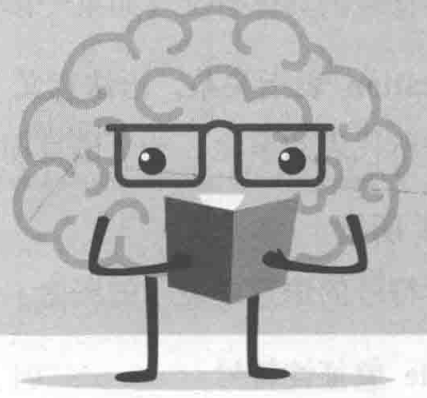
\includegraphics[width=.29\linewidth]{assets/partie2_illustration.png}\end{center}
\minititle{Le chapitre 7}
Phonétique articulatoire : ce chapitre répond à une question simple en apparence : comment produit-on les sons de notre langue ? Nous sommes en effet des êtres parlants qui émettons au quotidien des sons, mais de façon mécanique, sans en être vraiment conscients, un peu comme lorsque l’on respire. Ce chapitre a donc pour but de remettre de la conscience dans un processus quasi inconscient, et de lever les mystères de la voix.
\minititle{Le chapitre 8}
Phonologie : nous continuerons à nous intéresser aux sons de notre langue, mais du point de vue de leur fonction. Nous répondrons principalement à deux questions : comment fonctionne le langage ? Quelles sont ses fonctions ? On verra les travaux des savants du Cercle Linguistique de Prague, et notamment ceux Roman Jakobson et d’André Martinet,\ednote{原文 ceux Roman Jakobson 如此；应为 ceux de Roman Jakobson，与后面的 et d’André Martinet 对应。} célèbres pour leurs apports essentiels à la linguistique fonctionnelle.
\minititle{Le chapitre 9}
Après les phonèmes, les morphèmes feront l’objet du chapitre 9, Morphologie. Une partie non négligeable de ce chapitre sera consacrée à la morphologie lexicale. Nous répond à la question : comment fabrique-t-on des mots ?\ednote{原文 Nous répond 如此；现在时应为 Nous répondons；若与前句预告下文的将来时一致，则为 Nous répondrons。}
\minititle{Le chapitre 10}
Après avoir combiné phonèmes et morphèmes, il faut assembler les mots ainsi fabriqués pour construire des phrases. Ces mots vont dès lors entretenir différents types de rapports, qui seront présentés dans le chapitre 10, Syntaxe. Dans la deuxième partie de ce chapitre, je présenterai également une théorie syntaxique originale, la syntaxe structurale du linguiste français Lucien Tesnière, qui vous sera utile dans la troisième partie de notre livre.
\minititle{Le chapitre 11}
Construire des phrases, c’est bien. Construire des phrases dotées de sens, c’est mieux. Sens, signification, connotation, dénotation, sèmes, etc. feront l’objet du Chapitre 11, Sémantique, consacré à l’étude du sens. Nous y rencontrerons des linguistes et sémanticiens contemporains de tout premier plan, comme Louis Hjelmslev, Julien Greimas, Bernard Pottier ou encore François Rastier; et répondrons à la question : que veut-on dire avec les mots ?
\minititle{Le chapitre 12}
Les cinq chapitres précédents ont pour finalité un but bien pratique : celui de parler. L’étude de l’utilisation du langage fera l’objet du chapitre 12, Pragmatique. Centré autour de la théorie des actes de langages, ce chapitre abordera également la linguistique de l’énonciation, de la conversation, et de la politesse. Nous y répondrons à une question bien pratique : que peut-on faire avec des mots ?
